% Shared standalone design for the editable figure reconstructions.
\documentclass[tikz,border=5pt,10pt]{standalone}
\usepackage[T1]{fontenc}
\usepackage[utf8]{inputenc}
\usepackage{newpxtext,newpxmath}
\usepackage[scaled=.94]{sourcesanspro}
\usepackage{pgfplots}
\pgfplotsset{compat=1.18}
\usetikzlibrary{arrows.meta,calc,positioning,decorations.pathreplacing,
  decorations.markings,patterns,matrix,shapes.geometric,fit,backgrounds,
  intersections,angles,quotes}
\definecolor{ink}{HTML}{203746}
\definecolor{accent}{HTML}{146C78}
\definecolor{muted}{HTML}{667780}
\definecolor{signalred}{HTML}{B94B44}
\color{ink}
\tikzset{>=Latex,line width=.8pt,
  every node/.style={font=\small},
  axis/.style={->,draw=muted,line width=.5pt},
  guide/.style={draw=muted,dashed,line width=.45pt},
  curve/.style={draw=accent,line width=1pt},
  marker/.style={circle,fill=accent,inner sep=1.5pt},
  labelbox/.style={fill=white,inner sep=2pt}}

\begin{document}
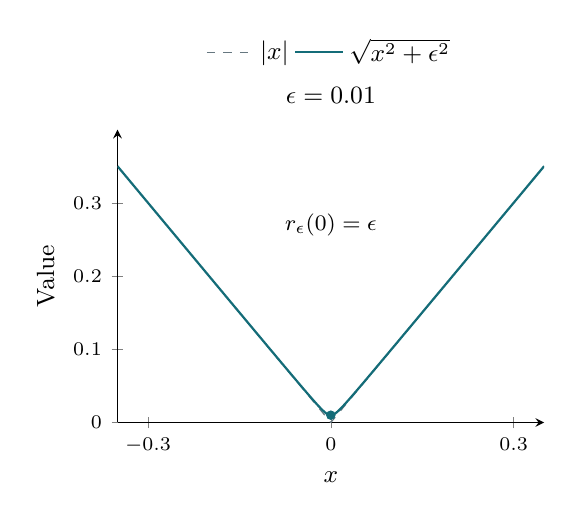
\begin{tikzpicture}
\begin{axis}[width=7cm,height=5.3cm,xmin=-.35,xmax=.35,ymin=0,ymax=.4,axis lines=left,xlabel={$x$},ylabel={Value},xtick={-.3,0,.3},ytick={0,.1,.2,.3},tick label style={font=\scriptsize},title={$\epsilon=0.01$},legend style={at={(.5,1.18)},anchor=south,draw=none,font=\footnotesize},legend columns=2]
\addplot[muted,dashed,domain=-.35:.35,samples=151] {abs(x)};\addlegendentry{$|x|$}
\addplot[accent,thick,domain=-.35:.35,samples=301] {sqrt(x*x+0.01^2)};\addlegendentry{$\sqrt{x^2+\epsilon^2}$}
\addplot[only marks,mark=*,accent,mark size=1.5pt,forget plot] coordinates {(0,0.01)};
\node[font=\footnotesize] at (axis cs:0,.27) {$r_\epsilon(0)=\epsilon$};
\end{axis}
\end{tikzpicture}
\end{document}
